\documentclass[12pt,a4paper]{article}

\usepackage[left=2.5cm,right=2.5cm,top=2.5cm,bottom=2.5cm]{geometry}
\usepackage[T1]{fontenc}
\usepackage[utf8]{inputenc}
\usepackage{amsmath}
\usepackage{amssymb}
\usepackage{graphicx}
\usepackage{tikz}
\usepackage{pgfplots}
\usepackage{booktabs}
\usepackage{url}
\usepackage{caption}
\usepackage{subcaption}
\usepackage{natbib}
\usepackage{hyperref}
\usepackage{xcolor}
\usepackage{cleveref}

% Packages for nice tables
\usepackage{multirow}
\usepackage{array}

% Hyperref setup
\hypersetup{
    colorlinks=true,
    linkcolor=blue,
    filecolor=magenta,
    urlcolor=cyan,
    citecolor=black
}

% Custom commands
\newcommand{\TODO}[1]{\textcolor{red}{TODO: #1}}
\newcommand{\B}[1]{\mathbf{#1}}
\newcommand{\norm}[1]{\|#1\|}

% Title
\title{Methodology and Implementation Details: Plain-DETR with DINOv3 for Object Detection on COCO Dataset}
\author{Experiment Report}
\date{\today}

\begin{document}

\maketitle

\section{Introduction}

This chapter describes the theoretical foundations and implementation details of the object detection experiment conducted using Plain-DETR with a DINOv3 Vision Transformer backbone on the COCO 2017 dataset. The experiment aims to evaluate a simplified detection transformer architecture that eliminates multi-scale feature processing while maintaining global cross-attention mechanisms for visual feature extraction. This section provides comprehensive details on the detection framework, the backbone architecture, the data processing pipeline, the tensor flow through the network, and the training configuration.

The object detection task in computer vision involves localizing and classifying objects within images. Traditional approaches relied on sliding window mechanisms and hand-crafted features, while modern deep learning methods employ convolutional neural networks for feature extraction. The introduction of transformers~\cite{vaswani2017attention} to computer vision, particularly through the Vision Transformer architecture~\cite{dosovitskiy2020image}, enabled modeling long-range dependencies across the entire image. DETR~\cite{carion2020end} pioneered end-to-end object detection with transformers, eliminating the need for non-maximum suppression and anchor generation. Plain-DETR further simplifies this approach by using single-scale features and global cross-attention, removing the multi-scale feature pyramids and deformable attention mechanisms required by original DETR.

\section{Plain-DETR Architecture}

Plain-DETR represents a simplified variant of the Detection Transformer architecture that eliminates several complex components from the original DETR framework while maintaining competitive detection performance. Unlike standard DETR that employs multi-scale features from a Feature Pyramid Network and deformable attention mechanisms, Plain-DETR operates on single-scale feature maps extracted from a Vision Transformer backbone and utilizes global cross-attention with relative position encodings.

\subsection{Overall Detection Pipeline}

The detection pipeline consists of five main stages. First, the input image undergoes preprocessing through data augmentation transforms. Second, the Vision Transformer backbone extracts feature representations from the preprocessed image. Third, an input projection layer maps the backbone features to the transformer's hidden dimension. Fourth, the decoder processes queries against the visual features through multi-head attention operations to generate predictions. Fifth, prediction heads produce class logits and bounding box coordinates.

The following pseudocode illustrates the complete forward pass through the Plain-DETR model:

\begin{verbatim}
# Input: batch of images
samples: NestedTensor[tensors=B×3×H×W, is_padding=B×H×W]

# Stage 1: Backbone feature extraction
features, pos = backbone(samples)
# features["0"]: B × C_backbone × (H/16) × (W/16)
# pos["0"]: B × C_backbone × (H/16) × (W/16)

# Stage 2: Input projection to hidden dimension
src = input_proj[0](features["0"].tensors)
# src: B × 256 × (H/16) × (W/16)

# Stage 3: Transformer decoder
hs, init_reference, inter_references = transformer(srcs, is_paddings, pos)
# hs: num_layers × B × num_queries × 256
# init_reference: B × num_queries × 2

# Stage 4: Prediction heads
outputs_class = class_embed[lvl](hs[lvl])
outputs_coord = bbox_embed[lvl](hs[lvl]) + reference
outputs_coord = outputs_coord.sigmoid()
\end{verbatim}

The model uses learnable query embeddings that are processed through the decoder layers. Each decoder layer refines the bounding box predictions through iterative box refinement, where the initial reference points are updated after each layer. This design allows the model to progressively localize objects with increasing accuracy.

\subsection{One-to-One and One-to-Many Matching}

Plain-DETR employs a hybrid matching strategy that combines one-to-one and one-to-many correspondence between predictions and ground truth objects. The one-to-one branch produces the final detection outputs and uses the Hungarian algorithm for optimal assignment. The one-to-many branch creates multiple predictions per ground truth object to provide stronger training signals during the learning process.

Let $N$ denote the number of one-to-one queries and $M$ denote the number of one-to-many queries. The total number of queries is $N + M$. The one-to-one queries produce the final outputs that are matched one-to-one with ground truth boxes using the Hungarian algorithm. The one-to-many queries generate additional predictions that are matched by expanding each ground truth object $k$ times, creating multiple positive assignments for enhanced supervision.

The loss function combines both branches:

\begin{equation}
\mathcal{L}_{total} = \mathcal{L}_{one2one} + \lambda \cdot \mathcal{L}_{one2many}
\end{equation}

where $\lambda$ is a weighting factor (set to 1.0 in our configuration).

\subsection{Global Cross-Attention with Relative Position Encoding}

The decoder employs global cross-attention rather than deformable attention. In global attention, each query attends to all position in the feature memory rather than a sparse set of sampling points. To incorporate positional information, relative position encodings are computed using learned MLP layers.

Given query features $Q$, key features $K$, and reference points $P_{ref}$, the attention computation proceeds as follows. First, reference points in pixel coordinates are computed as:

\begin{equation}
P_{pixel} = P_{ref} \cdot [W, H, W, H]
\end{equation}

where $W$ and $H$ are the feature map dimensions. Second, relative position offsets are computed between reference points and all spatial locations:

\begin{equation}
\delta_x = P_{pixel}[:, :, :, 0::2] - pos_x
\delta_y = P_{pixel}[:, :, :, 1::2] - pos_y
\end{equation}

Third, MLP layers transform these offsets into bias terms:

\begin{equation}
B_x = MLP_x(\delta_x), \quad B_y = MLP_y(\delta_y)
\end{equation}

Fourth, the final bias is $B = B_x + B_y$, which is added to the attention matrix before softmax. This relative position encoding allows the model to understand spatial relationships between queries and visual features without limiting attention to specific spatial locations.

\section{DINOv3 Vision Transformer Backbone}

The DINOv3 backbone is a Vision Transformer pretrained using self-distillation with no labels, following the DINO (Distillation with No Labels) framework. The backbone processes images as sequences of learnable patch embeddings, enabling global receptive fields and self-attention mechanisms across the entire feature map.

\subsection{ViT Architecture Fundamentals}

Vision Transformers partition an input image into fixed-size patches, linear embed each patch into a vector, and process the resulting sequence through transformer blocks. Let the input image be $X \in \mathbb{R}^{3 \times H \times W}$. First, the image is split into patches of size $16 \times 16$:

\begin{equation}
X_{patches} \in \mathbb{R}^{(HW/16^2) \times 3 \times 16 \times 16}
\end{equation}

Second, each patch is flattened and projected through a linear layer to the embedding dimension $D$:

\begin{equation}
E = Linear_{patch}(X_{patches}), \quad E \in \mathbb{R}^{N \times D}
\end{equation}

where $N = (H \cdot W) / 256$ is the number of patches.

Third, learnable position embeddings are added to each patch embedding to preserve spatial information:

\begin{equation}
E_{pos} = E + PE
\end{equation}

where $PE \in \mathbb{R}^{N \times D}$ is the learned position embedding.

Fourth, a learnable [CLS] token is prepended to the sequence for classification tasks:

\begin{equation}
E_{final} = [CLS] \oplus E_{pos}
\end{equation}

The sequence is then processed through $L$ transformer blocks, each containing multi-head self-attention followed by a feed-forward network with residual connections and layer normalization.

Each transformer block performs the following operations. The multi-head self-attention computes:

\begin{equation}
Q = W_Q E_{in}, \quad K = W_K E_{in}, \quad V = W_V E_{in}
\end{equation}

\begin{equation}
Attention(Q, K, V) = Softmax\left(\frac{QK^T}{\sqrt{D}}\right)V
\end{equation}

The feed-forward network applies:

\begin{equation}
FFN(E) = W_2(\sigma(W_1 E_{in} + b_1) + b_2)
\end{equation}

where $\sigma$ is the GELU activation function.

For the ViT-Small variant used in this experiment, the configuration is: patch size 16, embedding dimension 384, 12 transformer blocks, and 6 attention heads. The output stride is 16, meaning the spatial resolution of output features is reduced by a factor of 16 compared to the input image.

The following figure illustrates the ViT architecture:

\begin{figure}[htbp]
\centering
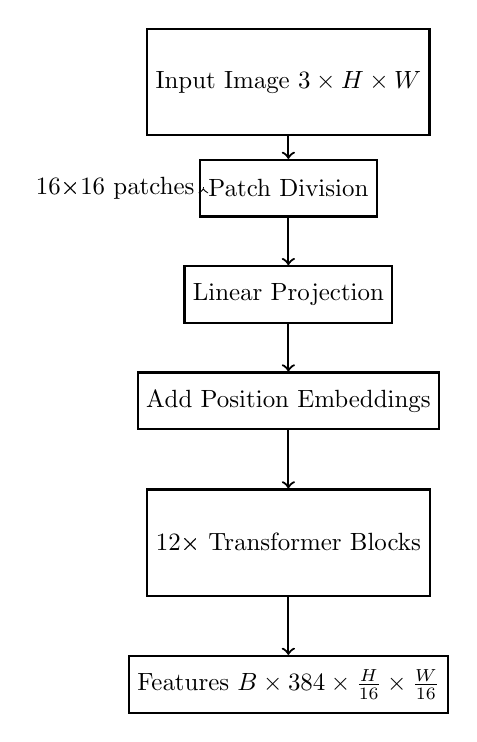
\begin{tikzpicture}[scale=0.9, every node/.style={scale=0.9}]

% Input image
\node[draw,thick,minimum width=2cm,minimum height=1.5cm] (input) at (0,0) {Input Image $3 \times H \times W$};

% Patching
\node[draw,thick,minimum width=2cm,minimum height=0.8cm] (patch) at (0,-1.5) {Patch Division};

% Linear embed
\node[draw,thick,minimum width=2cm,minimum height=0.8cm] (embed) at (0,-3) {Linear Projection};

% Add position
\node[draw,thick,minimum width=2cm,minimum height=0.8cm] (pos) at (0,-4.5) {Add Position Embeddings};

% Transformer blocks
\node[draw,thick,minimum width=4cm,minimum height=1.5cm] (trans) at (0,-6.5) {12× Transformer Blocks};

% Output
\node[draw,thick,minimum width=2cm,minimum height=0.8cm] (out) at (0,-8.5) {Features $B \times 384 \times \frac{H}{16} \times \frac{W}{16}$};

% Arrows
\draw[->,thick] (input.south) -- (patch.north);
\draw[->,thick] (patch.south) -- (embed.north);
\draw[->,thick] (embed.south) -- (pos.north);
\draw[->,thick] (pos.south) -- (trans.north);
\draw[->,thick] (trans.south) -- (out.north);

% Labels for patch size
\draw[->] (-1.2,-1.5) -- (-1.2,-1.5) node[left] {16×16 patches};

\end{tikzpicture}
\caption{Vision Transformer (ViT) Architecture: The input image is divided into 16×16 patches, linearly projected to the embedding dimension, position embeddings are added, and processed through 12 transformer blocks to produce single-scale features at stride 16.}
\end{figure}

The self-supervised pretraining of DINOv3 uses a teacher-student architecture. The teacher network processes the image with exponential moving average updates, while the student network learns to match the teacher's predictions. This approach enables the backbone to learn rich visual representations without manual annotations.

\section{Data Processing Pipeline}

The COCO 2017 dataset serves as the benchmark for object detection tasks. The dataset contains 118,287 training images and 5,000 validation images with 80 object categories. Each image may contain multiple object instances with corresponding bounding box annotations.

\subsection{Data Transforms}

The training pipeline applies a sequence of augmentations to increase model robustness. The transformation pipeline follows the order presented in the pseudocode:

\begin{verbatim}
# Training transforms (in order)
transforms = Compose([
    RandomHorizontalFlip(p=0.5),           # Horizontal flip with probability 0.5
    RandomSelect(                      # Randomly select one of two strategies
        Strategy_A: RandomResize(scales=[480,512,...,800], max_size=1333),
        Strategy_B: Compose([
            RandomResize([400, 500, 600]),
            RandomSizeCrop(384, 600),
            RandomResize(scales, max_size=1333)
        ])
    ),
    ToTensor(),                    # Convert PIL to FloatTensor [0,1]
    Normalize(mean=[0.485,0.456,0.406], std=[0.229,0.224,0.225])
])

# Validation transforms
transforms = Compose([
    RandomResize([800], max_size=1333),
    ToTensor(),
    Normalize(mean, std)
])
\end{verbatim}

The random horizontal flip increases training diversity by mirroring images with 50\% probability. The random resize operation scales images to random sizes between 480 and 800 pixels while maintaining aspect ratio. The random size crop provides additional viewpoint diversity by cropping a random region of size 384×600 before resizing. The ToTensor operation converts PIL images to floating-point tensors normalized to the [0,1] range. The normalization uses ImageNet statistics with mean [0.485, 0.456, 0.406] and standard deviation [0.229, 0.224, 0.225].

Box transformations convert coordinates from XYXY (top-left x, top-left y, bottom-right x, bottom-right y) to CXCYWH (center x, center y, width, height) format. The boxes are normalized by the image dimensions:

\begin{equation}
Box_{norm} = \frac{Box_{xyxy}}{[W, H, W, H]}
\end{equation}

This normalization ensures box coordinates are independent of absolute image sizes.

\subsection{NestedTensor for Batching}

Images in a batch have different spatial dimensions after augmentation. The NestedTensor structure handles variable-sized images by padding to the maximum dimensions within the batch and maintaining a binary mask indicating valid pixels. Let $B$ be the batch size, $C=3$ the number of channels, and $H_{max} \times W_{max}$ the maximum spatial dimensions:

\begin{equation}
NestedTensor.tensors \in \mathbb{R}^{B \times C \times H_{max} \times W_{max}}
\end{equation}

\begin{equation}
NestedTensor.is\_padding \in \mathbb{R}^{B \times H_{max} \times W_{max}}
\end{equation}

The padding mask contains True for padded regions and False for valid image content:

\begin{verbatim}
# Pseudocode for NestedTensor creation
def nested_tensor_from_tensor_list(tensor_list):
    num_images = len(tensor_list)
    max_channels = max(t.shape[0] for t in tensor_list)
    max_height = max(t.shape[1] for t in tensor_list)
    max_width = max(t.shape[2] for t in tensor_list)
    
    tensor = torch.zeros(B, max_channels, max_height, max_width)
    is_padding = torch.ones(B, max_height, max_width, dtype=torch.bool)
    
    for i, img in enumerate(tensor_list):
        c, h, w = img.shape
        tensor[i, :c, :h, :w] = img
        is_padding[i, :h, :w] = False
    
    return NestedTensor(tensor, is_padding)
\end{verbatim}

This structure ensures efficient batching while allowing variable input sizes.

\section{Training Configuration}

The experiment uses specific hyperparameters optimized for Plain-DETR with the DINOv3 backbone. The following table presents the complete configuration:

\begin{table}[htbp]
\centering
\caption{Training Configuration Parameters}
\label{tab:config}
\resizebox{\linewidth}{!}{
\begin{tabular}{lcc}
\toprule
\textbf{Parameter} & \textbf{Value} & \textbf{Description} \\
\midrule
Backbone & DINOv3-ViT-Small & Pretrained ViT with 21M parameters \\
Pretrained Weights Path & ./pt\_models/dinov3\_vit\_small.safetensors & Path to pretrained backbone \\
Batch Size (per GPU) & 8 & Training batch per GPU \\
Number of GPUs & 2 & Distributed training \\
Effective Batch Size & 16 & Total batch across GPUs \\
Epochs & 12 & Total training epochs \\
Learning Rate & $2 \times 10^{-4}$ & Initial learning rate \\
Learning Rate Drop & 11 & Epoch to reduce learning rate \\
Warmup Iterations & 1000 & Learning rate warmup phase \\
Weight Decay & 0.05 & Optimizer weight decay \\
Norm Type & pre\_norm & Layer normalization type \\
Dropout & 0.0 & Dropout rate \\
Drop Path Rate & 0.1 & Stochastic depth rate \\
Number of Feature Levels & 1 & Single-scale backbone output \\
Decoder Type & global\_rpe\_decomp & Global attention with RPE decomposition \\
Proposal Feature Levels & 4 & Multi-scale proposals for two-stage \\
Number of Queries (one-to-one) & 300 & Detection queries \\
Number of Queries (one-to-many) & 1500 & Auxiliary queries \\
k (one-to-many) & 6 & Positive matches per ground truth \\
Lambda (one-to-many weight) & 1.0 & Weight for one-to-many loss \\
Use Layerwise Decay & True & Different LR per layer \\
LR Decay Rate & 0.9 & Layer-wise decay factor \\
\bottomrule
\end{tabular}
}
\end{table}

The configuration employs several training techniques. The layer-wise learning rate decay applies decreasing learning rates to deeper layers:

\begin{equation}
LR_{layer_i} = LR_{base} \cdot \gamma^{i}
\end{equation}

where $\gamma = 0.9$ is the decay rate and $i$ is the layer index.

The warmup phase gradually increases the learning rate from zero to the target value over the first 1000 iterations. After warmup, the learning rate follows a step schedule:

\begin{equation}
LR(epoch) = 
\begin{cases}
LR_{base} & \text{if } epoch < epoch_{drop} \\
LR_{base} \cdot 0.1 & \text{if } epoch \geq epoch_{drop}
\end{cases}
\end{equation}

The learning rate drops by a factor of 10 after epoch 11 to enable finer convergence.

The training uses mixed precision with automatic differentiation disabled (FP32) to maintain numerical stability with the large transformer model.

\section{Tensor Flow Through the Network}

This section provides detailed tensor dimensions at each stage of the forward pass, tracking the transformation from input image to final predictions.

\subsection{Stage 1: Input and Backbone}

Input images first undergo transformation to NestedTensor format:

\begin{equation}
\text{Input: } \B{X} \in \mathbb{R}^{B \times 3 \times H \times W}
\end{equation}

After padding to the maximum dimensions in batch:

\begin{equation}
\text{NestedTensor.tensors: } \B{X}_{pad} \in \mathbb{R}^{B \times 3 \times H_{max} \times W_{max}}
\end{equation}

The backbone processes the padded tensor through the ViT model and produces single-scale features:

\begin{equation}
\B{F}_{backbone} \in \mathbb{R}^{B \times C_{back} \times \frac{H}{16} \times \frac{W}{16}}
\end{equation}

For DINOv3-ViT-Small, $C_{back} = 384$. The stride is 16 because the patch size is 16.

Pseudocode describing this stage:

\begin{verbatim}
# Backbone forward
features, pos = backbone(samples.tensors, samples.is_padding)
# features["0"]: B × 384 × (H/16) × (W/16)
# pos["0"]: B × 384 × (H/16) × (W/16)
\end{verbatim}

\subsection{Stage 2: Input Projection}

A 1×1 convolution followed by GroupNorm projects the backbone features to the transformer's hidden dimension:

\begin{equation}
\B{F}_{proj} = \text{Conv}_{1\times1}(\B{F}_{backbone}) + \text{GroupNorm}(\B{F}_{backbone})
\end{equation}

\begin{equation}
\B{F}_{proj} \in \mathbb{R}^{B \times D \times \frac{H}{16} \times \frac{W}{16}}
\end{equation}

where $D = 256$ is the hidden dimension used throughout the transformer.

The projection does not change spatial dimensions because it uses 1×1 kernels:

\begin{verbatim}
src = input_proj[0](features["0"].tensors)
# src: B × 256 × (H/16) × (W/16)
\end{verbatim}

\subsection{Stage 3: Feature Flattening}

For the transformer, features are flattened to sequence format. Let $S = \frac{H}{16} \cdot \frac{W}{16}$ be the sequence length:

\begin{equation}
\B{F}_{seq} = \text{Flatten}_{spatial}(\B{F}_{proj}) \in \mathbb{R}^{B \times S \times D}
\end{equation}

Position embeddings are similarly flattened:

\begin{equation}
\B{P}_{seq} = \text{Flatten}_{spatial}(\B{P}) \in \mathbb{R}^{B \times S \times D}
\end{equation}

Spatial shapes are preserved for attention computations:

\begin{verbatim}
# Flattening
src_flatten = src.flatten(2).transpose(1, 2)  # B × S × 256
is_padding_flatten = is_padding.flatten(1)    # B × S
pos_flatten = pos_embed.flatten(2).transpose(1, 2)  # B × S × 256
spatial_shapes = [(H/16, W/16)]
\end{verbatim}

\subsection{Stage 4: Query Initialization}

Learnable query embeddings are initialized for one-to-one and one-to-many branches. The total query dimension is $Q_{total} = Q_{one2one} + Q_{one2many} = 300 + 1500 = 1800$:

\begin{equation}
\B{Q}_{embed} \in \mathbb{R}^{Q_{total} \times 2D}
\end{equation}

The 2D embeddings are split into content queries ($tgt$) and position queries ($query\_pos$):

\begin{equation}
tgt, query\_pos = \text{split}(\B{Q}_{embed}, D)
\end{equation}

Reference points start as normalized coordinates:

\begin{verbatim}
# Query initialization
query_embed = nn.Embedding(num_queries, hidden_dim * 2)
query_embed, tgt = torch.split(query_embed.weight, hidden_dim, dim=1)
# query_embed: [num_queries, 256]
# tgt: [num_queries, 256]

# Expand to batch
query_embed = query_embed.unsqueeze(0).expand(B, -1, -1)  # B × num_queries × 256
tgt = tgt.unsqueeze(0).expand(B, -1, -1)        # B × num_queries × 256

# Initial reference points
reference_points = reference_points(query_embed).sigmoid()  # B × num_queries × 2
\end{verbatim}

For the two-stage mode (enabled in configuration), initial reference points come from encoder proposals:

\begin{verbatim}
reference_points = encoder_proposals.sigmoid()  # B × num_proposals × 2
\end{verbatim}

The reference points are in normalized [0,1] coordinate format representing center coordinates.

\subsection{Stage 5: Decoder Layers}

Each decoder layer performs self-attention followed by global cross-attention to the encoder memory, then a feed-forward network:

\begin{verbatim}
# Decoder layer l
# 1. Self-attention
tgt = self.self_attn(tgt, tgt, tgt, attn_mask=self_attn_mask)

# 2. Cross-attention with global RPE
tgt = self.cross_attn(
    query=tgt, 
    key=memory,           # encoder features
    value=memory,
    rpe_attn=bias       # relative position encoding bias
)

# 3. Feed-forward network
tgt = self.ffn(tgt)
\end{verbatim}

The decoder outputs hidden states at each layer:

\begin{equation}
\B{H}_{l} \in \mathbb{R}^{B \times Q_{total} \times D} \quad \text{for } l = 0, \ldots, L-1
\end{equation}

Reference points are refined after each layer:

\begin{equation}
\B{R}_{l} = \sigma(\B{R}_{l-1} + \Delta\B{R}_{l})
\end{equation}

where $\sigma$ is the sigmoid function and $\Delta\B{R}$ is the predicted offset.

Each decoder layer processes the tensors with these dimensions. The input comprises hidden states $[B, Q_{total}, 256]$, reference points $[B, Q_{total}, 2]$, memory $[B, S, 256]$, and position embeddings $[B, S, 256]$. The outputs include refined hidden states $[B, Q_{total}, 256]$ and refined reference points $[B, Q_{total}, 2]$.

The following figure shows the decoder architecture:

\begin{figure}[htbp]
\centering
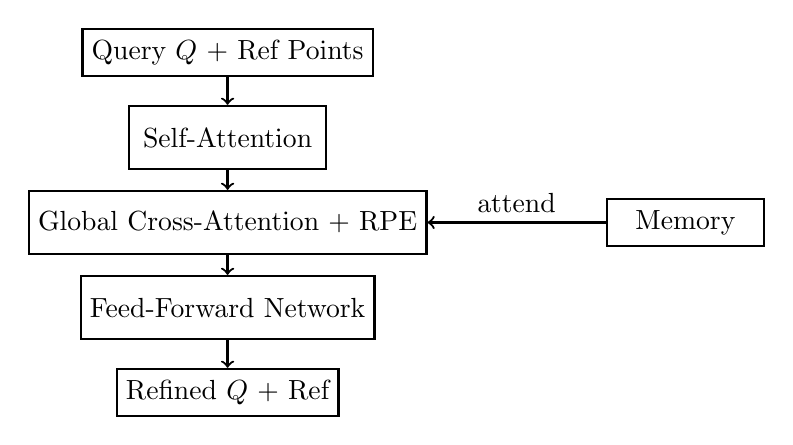
\begin{tikzpicture}[scale=0.9]

% Input
\node[draw,thick,minimum width=2cm,minimum height=0.6cm] (input) at (0,0) {Query $Q$ + Ref Points};

% Self-attention
\node[draw,thick,minimum width=2.5cm,minimum height=0.8cm] (selfattn) at (0,-1.2) {Self-Attention};

% Cross-attention  
\node[draw,thick,minimum width=2.5cm,minimum height=0.8cm] (crossattn) at (0,-2.4) {Global Cross-Attention + RPE};

% FFN
\node[draw,thick,minimum width=2.5cm,minimum height=0.8cm] (ffn) at (0,-3.6) {Feed-Forward Network};

% Output
\node[draw,thick,minimum width=2cm,minimum height=0.6cm] (output) at (0,-4.8) {Refined $Q$ + Ref};

% Memory
\node[draw,thick,minimum width=2cm,minimum height=0.6cm,right=3cm] (memory) at (2,-2.4) {Memory};

% Arrows
\draw[->,thick] (input.south) -- (selfattn.north);
\draw[->,thick] (selfattn.south) -- (crossattn.north);
\draw[->,thick] (crossattn.south) -- (ffn.north);
\draw[->,thick] (ffn.south) -- (output.north);
\draw[->,thick] (memory.west) -- (crossattn.east) node[midway,above] {attend};

\end{tikzpicture}
\caption{Decoder Layer Architecture: Each layer consists of self-attention on queries, global cross-attention to encoder memory with relative position encoding, and a feed-forward network. The reference points are refined after each layer.}
\end{figure}

The decoder consists of six layers by default (configurable through the model architecture).

The final decoder output is:

\begin{equation}
\B{H} \in \mathbb{R}^{L \times B \times Q \times D} \quad \text{and} \quad \B{R} \in \mathbb{R}^{L \times B \times Q \times 2}
\end{equation}

where $L$ is the number of decoder layers.

\subsection{Stage 6: Prediction Heads}

Linear projection layers produce class logits and bounding box coordinates from the decoder outputs. For each decoder layer $l$:

\begin{equation}
\B{Logits}_{l} = \text{Linear}(\B{H}_{l}) \in \mathbb{R}^{B \times Q \times (C+1)}
\end{equation}

\begin{equation}
\B{BoxDelta}_{l} = \text{Linear}(\B{H}_{l}) \in \mathbb{R}^{B \times Q \times 4}
\end{equation}

where $C=91$ is the number of COCO classes (including background as extra class).

The box predictions are added to reference points and transformed through sigmoid:

\begin{equation}
\B{Box}_{l} = \sigma(\B{BoxDelta}_{l} + \B{R}_{l}) \in \mathbb{R}^{B \times Q \times 4}
\end{equation}

The box format is normalized center-width-height (cx, cy, w, h) in [0,1] range.

One-to-one outputs use the first 300 queries; one-to-many outputs use the remaining 1500 queries:

\begin{verbatim}
# Split outputs
outputs_class_o2o = outputs_class[:, 0:300]     # B × 300 × 92
outputs_coord_o2o = outputs_coord[:, 0:300]     # B × 300 × 4
outputs_class_o2m = outputs_class[:, 300:1800]   # B × 1500 × 92
outputs_coord_o2m = outputs_coord[:, 300:1800]   # B × 1500 × 4
\end{verbatim}

The final predictions have these dimensions: class logits $[B, 300, 92]$ (91 classes plus background) and bounding boxes $[B, 300, 4]$ (cx, cy, w, h normalized).

The complete tensor flow summary appears in the following table:

\begin{table}[htbp]
\centering
\caption{Tensor Dimensions Throughout the Network}
\label{tab:tensors}
\begin{tabular}{lll}
\toprule
\textbf{Stage} & \textbf{Tensor} & \textbf{Dimensions} \\
\midrule
Input & $\B{X}$ & $B \times 3 \times H \times W$ \\
Backbone Output & $\B{F}_{backbone}$ & $B \times 384 \times \frac{H}{16} \times \frac{W}{16}$ \\
Input Projection & $\B{F}_{proj}$ & $B \times 256 \times \frac{H}{16} \times \frac{W}{16}$ \\
Flattened Features & $\B{F}_{seq}$ & $B \times S \times 256$ \\
Query Embeddings & $\B{Q}$ & $Q_{total} \times 512$ \\
Decoder Output & $\B{H}$ & $L \times B \times Q_{total} \times 256$ \\
Reference Points & $\B{R}$ & $L \times B \times Q_{total} \times 2$ \\
Class Logits & $\B{Logits}$ & $B \times Q_{one2one} \times 92$ \\
Bounding Boxes & $\B{Box}$ & $B \times Q_{one2one} \times 4$ \\
\bottomrule
\end{tabular}
\end{table}

Here $B=16$ (effective batch size), $H, W$ are input dimensions (variable), $S = \frac{H}{16} \cdot \frac{W}{16}$, $Q_{total} = 1800$, $Q_{one2one} = 300$, and $L$ is the number of decoder layers.

\section{Loss Functions}

The training loss combines four components computed through the Hungarian matching algorithm for optimal assignment.

The classification loss uses Focal Loss to handle the class imbalance:

\begin{equation}
\mathcal{L}_{cls} = -\alpha (1-p_t)^\gamma \log(p_t) - (1-\alpha) p_t^\gamma \log(1-p_t)
\end{equation}

with $\alpha = 0.25$ and $\gamma = 2.0$.

The bounding box loss uses $L_1$ loss on the normalized coordinates:

\begin{equation}
\mathcal{L}_{bbox} = \|\B{Box}_{pred} - \B{Box}_{gt}\|_1
\end{equation}

The Generalized IoU loss provides rotation-invariant box comparison:

\begin{equation}
\mathcal{L}_{giou} = 1 - \text{GIoU}(\B{Box}_{pred}, \B{Box}_{gt})
\end{equation}

where GIoU incorporates both intersection over union and the areaRatio between the union and enclosed bounding box.

The total loss combines these:

\begin{equation}
\mathcal{L}_{total} = \lambda_{cls}\mathcal{L}_{cls} + \lambda_{bbox}\mathcal{L}_{bbox} + \lambda_{giou}\mathcal{L}_{giou}
\end{equation}

with weights $\lambda_{cls} = 2$, $\lambda_{bbox} = 5$, and $\lambda_{giou} = 2$.

The matching process uses the Hungarian algorithm to solve the linear assignment problem:

\begin{verbatim}
# Hungarian matching
cost_matrix = cost_class × cost_class + 
             cost_bbox × cost_bbox + 
             cost_giou × cost_giou
            
indices = linear_sum_assignment(cost_matrix)
# Returns matched (query_idx, target_idx) pairs
\end{verbatim}

This ensures each ground truth object is matched to exactly one prediction during training.

\section{Evaluation Metrics}

The COCO dataset employs mean Average Precision (mAP) as the primary evaluation metric. The metric measures detection performance across different Intersection over Union thresholds.

The IoU threshold determines whether a prediction is considered correct. A prediction is a true positive if:

\begin{equation}
\text{IoU}(\B{Box}_{pred}, \B{Box}_{gt}) \geq IoU_{threshold}
\end{equation}

The AP metric is computed across IoU thresholds $\{0.50, 0.55, 0.60, \ldots, 0.95\}$ and averaged:

\begin{equation}
AP = \frac{1}{10} \sum_{t=0.5}^{0.95} AP_t
\end{equation}

The following table reports standard COCO metrics:

\begin{table}[htbp]
\centering
\caption{COCO Evaluation Metrics}
\label{tab:metrics}
\begin{tabular}{ll}
\toprule
\textbf{Metric} & \textbf{Description} \\
\midrule
AP & Average Precision across IoU=[0.5:0.95] \\
AP50 & AP at IoU=0.50 (PASCAL VOC metric) \\
AP75 & AP at IoU=0.75 (strict metric) \\
APs & AP for small objects (area < 32²) \\
APm & AP for medium objects (32² < area < 96²) \\
APl & AP for large objects (area > 96²) \\
\bottomrule
\end{tabular}
\end{table}

Evaluation runs after each training epoch on the validation set. The model with the best AP on the validation set is saved for final inference.

The evaluation pseudocode:

\begin{verbatim}
# Evaluation loop
for image, targets in validation_loader:
    predictions = model(image)
    
    # Filter by confidence threshold
    keep = predictions["pred_logits"].sigmoid() > 0.05
    
    # Compute IoU with ground truth
    iou = box_iou(predictions["pred_boxes"], targets["boxes"])
    
    # Accumulate for AP computation
    coco_eval.update(predictions, targets)

# Final metrics
coco_eval.synchronize()
coco_eval.accumulate()
coco_eval.summarize()
\end{verbatim}

The model evaluation produces metrics after each epoch, allowing tracking of detection performance improvements throughout training.

\section{Conclusion}

This chapter provided comprehensive details on the Plain-DETR architecture with DINOv3 backbone for object detection. The methodology covers the Vision Transformer backbone for feature extraction, single-scale processing with global cross-attention, the training configuration with all hyperparameters, detailed tensor dimensions through the network, loss functions for optimization, and evaluation metrics for performance assessment.

The experiment combines modern self-supervised representations (DINOv3) with a simplified detection transformer (Plain-DETR), eliminating multi-scale feature pyramids while maintaining global attention for spatial reasoning. This configuration represents a principled approach to efficient transformer-based object detection.

\bibliographystyle{plainnat}
\bibliography{references}

\end{document}